% -*- latex -*-

%%%%%%%%%%%%%%%%%%%%%%%%%%%%%%%%%%%%%%%%%%%%%%%%%%%%%%%%%%%%%%%%%%%%%%%%%%%%%
% This beginning part of the preamble is psecific to the IEEEtran document
% class.

\documentclass[conference]{IEEEtran}

%% \author{
%%   \IEEEauthorblockN{Kenneth~Moreland}
%%   \IEEEauthorblockA{Sandia National Laboratories\\
%%     Albuquerque, NM 87185-1326\\
%%     Email: kmorel@sandia.gov}
%%   \and
%%   \IEEEauthorblockN{Others}
%%   \IEEEauthorblockA{Cool Group\\
%%     Somewhere, WQ 12341\\
%%     Email: person@myspace.com}
%% }

\author{
  \IEEEauthorblockN{
    Kenneth~Moreland\IEEEauthorrefmark{1},
    Brad~King\IEEEauthorrefmark{2},
    Robert~Maynard\IEEEauthorrefmark{2}, and
    Kwan-Liu~Ma\IEEEauthorrefmark{3}
  }
  \IEEEauthorblockA{
    \IEEEauthorrefmark{1}Sandia National Laboratories,
    Albuquerque, NM 87185-1326}
  \IEEEauthorblockA{
    \IEEEauthorrefmark{2}Kitware, Inc.,
    Clifton Park, NY 12065}
  \IEEEauthorblockA{
    \IEEEauthorrefmark{3}Computer Science Department,
    University of California at Davis,
    Davis, CA 95616-8562}
}

% for over three affiliations, or if they all won't fit within the width
% of the page, use this alternative format:
% 
%\author{\IEEEauthorblockN{Michael Shell\IEEEauthorrefmark{1},
%Homer Simpson\IEEEauthorrefmark{2},
%James Kirk\IEEEauthorrefmark{3}, 
%Montgomery Scott\IEEEauthorrefmark{3} and
%Eldon Tyrell\IEEEauthorrefmark{4}}
%\IEEEauthorblockA{\IEEEauthorrefmark{1}School of Electrical and Computer Engineering\\
%Georgia Institute of Technology,
%Atlanta, Georgia 30332--0250\\ Email: see http://www.michaelshell.org/contact.html}
%\IEEEauthorblockA{\IEEEauthorrefmark{2}Twentieth Century Fox, Springfield, USA\\
%Email: homer@thesimpsons.com}
%\IEEEauthorblockA{\IEEEauthorrefmark{3}Starfleet Academy, San Francisco, California 96678-2391\\
%Telephone: (800) 555--1212, Fax: (888) 555--1212}
%\IEEEauthorblockA{\IEEEauthorrefmark{4}Tyrell Inc., 123 Replicant Street, Los Angeles, California 90210--4321}}

% End of IEEEtran-specific portion of the preamble.
%%%%%%%%%%%%%%%%%%%%%%%%%%%%%%%%%%%%%%%%%%%%%%%%%%%%%%%%%%%%%%%%%%%%%%%%%%%%%


\usepackage{amsfonts}
\usepackage{amssymb}
\usepackage{amsmath}
\usepackage{graphicx}
\usepackage{varioref}
\usepackage{fancyvrb}
\usepackage{ifthen}
\usepackage{cite}
\usepackage{subfig}
\usepackage{xspace}
\usepackage[pdfborder={0 0 0}]{hyperref}
\usepackage{verbatim}

\usepackage{color}
\definecolor{yellow}{rgb}{1,1,0}
\definecolor{black}{rgb}{0,0,0}
\definecolor{ltcyan}{rgb}{.75,1,1}
\definecolor{red}{rgb}{1,0,0}
\definecolor{gray}{rgb}{.6,.6,.6}

% Cite commands I use to abstract away the different ways to reference an
% entry in the bibliography (superscripts, numbers, dates, or author
% abbreviations).  \scite is a short cite that is used immediately after
% when the authors are mentioned.  \lcite is a full citation that is used
% anywhere.  Both should be used right next to the text being cited without
% any spacing.
\newcommand*{\lcite}[1]{~\cite{#1}}
\newcommand*{\scite}[1]{~\cite{#1}}

\newcommand{\etal}{et al.}

\newcommand*{\keyterm}[1]{\emph{#1}}

% Code highlighting markup.
\newcommand{\Ck}[1]{{#1}} % Language keyword
\newcommand{\Ci}[1]{{\textbf{#1}}} % Dax-provided identifier
\newcommand{\CiDesc}{\Ci{Bold}}
\newcommand{\Cu}[1]{{\color{gray}\textbf{#1}}} % User-provided identifier
\newcommand{\Code}[1]{{\small\texttt{#1}}}

\newcommand{\fix}[1]{{\color{red}\textsc{[#1]}}}

% Avoid putting figures on their own page.
\renewcommand{\textfraction}{0.05}
\renewcommand{\topfraction}{0.95}
\renewcommand{\bottomfraction}{0.95}

% Make sure this is big enough so that only big figures end up on their own
% page but small enough so that if a figure does have to be on its own
% page, it won't push everything to the bottom because it's not big enough
% to have its own page.
\renewcommand{\floatpagefraction}{.75}

\newenvironment{packed_itemize}{
\begin{itemize}
  \setlength{\topsep}{0pt}
  \setlength{\itemsep}{0pt}
  \setlength{\parskip}{0pt}
  \setlength{\parsep}{0pt}
  \setlength{\partopsep}{0pt}
}{\end{itemize}}

\title{Flexible Analysis Software for Emerging Architectures}

\hyphenation{Para-View Map-Re-duce}

\begin{document}

\sloppy

\maketitle

\begin{abstract}
  We are on the threshold of a transformative change in the basic
  architecture of high-performance computing.  The use of accelerator
  processors, characterized by large core counts, shared but asymmetrical
  memory, and heavy thread loading, is quickly becoming the norm in high
  performance computing.  These accelerators represent significant
  challenges in updating our existing base of software.  An intrinsic
  problem with this transition is a fundamental programming shift from
  message passing processes to much more fine thread scheduling with memory
  sharing.  Another problem is the lack of stability in accelerator
  implementation; processor and compiler technology is currently changing
  rapidly.  In this paper we describe our approach to address these two
  immediate problems with respect to scientific analysis and visualization
  algorithms.  Our approach to accelerator programming forms the basis of
  the Dax toolkit, a framework to build data analysis and visualization
  algorithms applicable to exascale computing.
\end{abstract}

\section{Introduction}
\label{sec:Introduction}

\noindent
Whereas supercomputers throughout the terascale era were almost
unilaterally built from general purpose CPU processors on distributed
memory nodes with a message passing interface, in petascale computing we
are seeing the emerging use of accelerators to meet the execution and
computation requirements of modern leadership-class facilities.  This trend
was kicked off when the Roadrunner supercomputer, first to achieve a
petaFLOP, was built with Cell BE processors\lcite{Henning2009}.  At the
time, Roadrunner was an anomaly, but since then many high-performance
computers followed this example.  Today, over 10\% of the Top 500
supercomputers incorporate accelerators, and that number is
growing.\footnote{According to the $39^{\mathrm{th}}$ edition of the Top500
  list of the world's supercomputers released June 18, 2012.  Available from
  \href{http://www.top500.org}{http://www.top500.org}.}

These accelerators represent a significant departure from how we most often
perform parallel processing.  Computing on the previous generation of high
performance computers involved partitioning data among distributed memory
nodes and running independent processes that pass messages.  However,
accelerators do not work well with such an approach.  Threads on an
accelerator may be grouped in SIMD ``warps,'' can have indeterminate
scheduling, and may be incapable of direct message passing\lcite{Sanders2011}.
Even on processors with more complete and independent cores, taking
advantage of shared memory threads can have its
advantages\lcite{Camp2010,Howison2011}.  Ultimately, our algorithms must
exhibit a more ``pervasive parallelism'' comprising a marked increase in
concurrency and careful data
management\lcite{ScientificDiscoveryExascale2011,ExascaleRoadMap}.

Another problem facing current research and development is the shifting
landscape of the development environment.  The Cell BE processors (and
associated compiler environment) comprising Roadrunner is already
discontinued.  Instead, NVIDIA is aggressively pursing leadership in
accelerator technology for scientific computation with Intel hot on its
heels.  Several compiler technologies such as OpenMP, CUDA, Threaded
Building Blocks, and OpenACC also compete for multi-threaded programming.

Our team is creating the Dax toolkit\lcite{Moreland2011:LDAV}, which seeks
to provide a development framework for scientific data analysis and
visualization algorithms for the next generation of high-performance
computers and beyond.  In this paper we document the following features.
\begin{itemize}
\item A general approach to data analysis and visualization algorithm
  development that provides a pervasive parallelism without the complexity
  of parallel programming.
\item An adapter mechanism that encapsulates the change in behavior
  required to port the toolkit among devices and compilers.
\item A concept-enabled mechanism to automatically build parallel
  scheduling code from signatures using C++ templates.
\end{itemize}

\section{Previous Work}
\label{sec:PreviousWork}

\noindent
To implement algorithms that are configurable with respect to operations,
data structures, and processor idiosyncrasies, Dax relies on
well-established techniques of generic programming\lcite{Musser1996}.
Generic programming uses C++ templates to direct the compiler to specialize
a particular piece of code to alternate implementations.

To maximize the amount of code that has no parallel dependencies, Dax
employs a functor-based execution mode\lcite{Baker2010}.  The intention of
this approach is to write a sequential section of code that operates on a
small section of data as a functional object, and then schedule this
function in parallel independently on large vector components.  The
technique can be thought of as a generalization of the map and reduce
operations in a MapReduce\lcite{MapReduce} framework.

A toolkit with similar goals of simplifying many-core parallel programming
and cross-device porting is Thrust\lcite{Thrust}.  Thrust is a more general
template library that provides a number of generic parallel algorithms.
Thrust provides many of the desired attributes of Dax and is in fact used
to implement many of them.  What differentiates Dax is the simplification
and specialization of its interface.  We can provide generic algorithms and
classes designed specifically for data analysis and visualization as well
as better specialize the data management.

It should be noted that this paper does not cover message passing,
distributed memory, or ``hybrid'' parallelism.  Although this is clearly
important in high-performance computing, the scope of this paper is only on
the shared-memory, many-core parallelism part of this problem.  The
techniques discussed here can be coupled with existing distributed memory
approaches\lcite{Ahrens2000,Peterka2011} to complete the hybrid parallelism
required to run concurrently across an entire machine.

\section{Algorithmic Approach}
\label{sec:AlgorithmicApproach}

\noindent
Our basic approach to building algorithms is to build kernels of execution
as functors.  These functors are designed to operate on a small element of
data in a serial and stateless manner.  Because this kernel does work on a
small amount of data, we call it a \keyterm{worklet}.  Around this concept,
we build a system to concurrently schedule these worklets across multiple
elements of a vector.

This approach mirrors that of Baker \etal\scite{Baker2010}.  Both
approaches use C++ templating to generically apply functors in parallel to
vectors of data.  Where our work significantly differs from that of Baker's
is in that we are more focused on the computational geometry problems
related to scientific visualization and data analysis.

Where Baker provides a simple mapping mechanism onto a vector, our system
is designed to provide a variety of parallel scheduling operations.  These
result in worklet types that get scheduled in different ways.  Each worklet
type has a different set of capabilities.  The current set of worklet types
are

\begin{description}[\IEEEsetlabelwidth{\quad}]
\item[Field Map]~\\ The Field Map is functionally equivalent to Baker's
  functional approach.  It applies a worklet operation independently and in
  parallel to each entry in one or more field arrays.
\item[Cell Map]~\\ The Cell Map is similar to the Field Map in functionally
  except that it takes the topology of the mesh into consideration.  The
  worklet is applied to each cell in the mesh and has access to any data,
  including point fields, on that cell.  This map enables operations that
  must interpolate across the cell.
\item[Topology Generator]~\\ The Topology Generator works similarly to the
  Cell Map with the exception that instead of creating a new field, it
  creates a new topology (that is, new cells).  One of the prerequisites of
  invoking a Topology Generator is a classification of how many new cells
  will be generated for each of the input cells.  This could be a constant
  value (which would be typical for a tetrahedralization), or it might be
  different for each input cell (which would be typical for operations like
  threshold or contour) and captured in an array.
\item[Point Reduction]~\\ A Point Reduction operation collects values
  associated with a vertex in the mesh and performs an operation that
  reduces to a single value.  Point Reduction has two primary uses.  First,
  when topology generation creates new vertices, field and other
  information can be reduced to the new point.  Second, a point reduction
  can gather information about all of its incident cells, which can be used
  to interpolate fields created with a Cell Map.
\end{description}

A common theme among all of the worklet types is their behavior of applying
the same operation across many small elements.  This approach is well
proven to be an efficient mechanism to drive many compute cores
simultaneously.

\section{Device Adapter}
\label{sec:DeviceAdapter}

\noindent
As multiple vendors vie to provide accelerator-type processors, a great
variance in the computer architecture exists, and we expect to encounter
further changes in the near future.  Likewise, there exist multiple
compiler environments and libraries for these devices.  The most popular of
these include OpenMP, CUDA, and OpenCL (although the latter does not yet
support C++ classes and templates).  These compiler technologies also vary
from system to system.

Consequently, we require our Dax toolkit to easily port from one system to
the next.  At a minimum, we require a base language support, and the
language we choose to support is C++.  The majority of the code in Dax is
constrained to the standard C++ language constructs to minimize the
specialization from one system to the next.

\begin{figure}[htb]
  \centering
  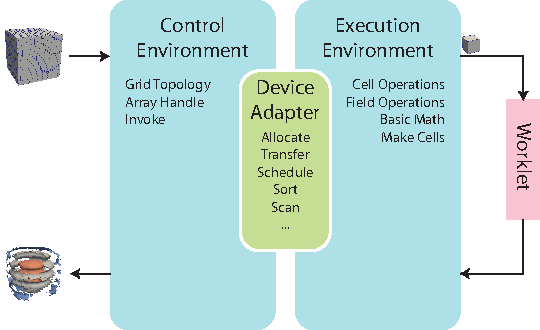
\includegraphics[width=\linewidth]{images/DaxDiagram}
  \caption{Diagram of the Dax framework.}
  \label{fig:DaxDiagram}
\end{figure}

Figure~\ref{fig:DaxDiagram} provides an overall diagram of the Dax
framework.  Dax is split into two environments, each with its own API.  The
\keyterm{control environment} is used to describe data, interface with
other libraries, and invoke parallel operations.  The control environment
is designed to run in a single thread within a process.  Parallel
algorithms are run in the \keyterm{execution environment}.  Worklets are
built using the execution environment API, which constrains their
operations to a safe region of data.

The control and execution environments are logically equivalent to the host
and device environments, respectively, in CUDA.  When compiling with CUDA,
these environments mirror each other, but the same logical approach is
taken when no such physical separation exists.

In between these two environments sits the \keyterm{device adapter}.  The
device adapter encapsulates all the specialized code required for running
on a particular device with a particular compiler technology.  The
functionality of the device adapter comprises two main parts: a collection
of parallel algorithms and a module to transfer data between the control
and execution environments.

Each device adapter is expected to implement a set algorithms containing
parallel for, scan, lower bounds (parallel find), stream compact, and unique
(remove duplicates).  This list of operations is similar to those suggested
by Blelloch\scite{Blelloch1990} and also a subset of those provided by the
Thrust library\lcite{Thrust}.  Thrust itself provides a convenient
implementation for device adapters because it itself is portable among
devices.  However, the interface to the device adapter algorithms is
independent of Thrust, and we have an example of a device adapter that can
be built without Thrust.

A device adapter also provides a module to handle the transfer of data
between the control and execution environments.  Unlike other systems such as
CUDA and Thrust, which explicitly define separate arrays and copy between
them, the Dax device adapter allocates and copies data in one monolithic
operation.  The advantage of this approach is that a device adapter for a
system that shares memory between the two environments (such as with
OpenMP) can perform shallow copies to share the data.

With these basic device adapter facilities, we can build a support library
for visualization algorithms.  Because the interface for the device adapter
is independent of the implementation for each device, this support library
can be built in such a way to be portable across many devices.

\section{Generic Array Handle}
\label{sec:GenericArrayHandle}

\noindent
The data model for Dax is deliberately simple.  The basic data container in
Dax is an \keyterm{array handle}.  The array handle acts like a smart
pointer to the data to manage its resource usage.  Array handle objects
maintain a reference count of how many instances point to the same array.

Array handle objects can also allocate and de-allocate data as necessary.
For example, when an array handle is used to store the output of an
algorithm, Dax will automatically allocate data in the array to store the
appropriate amount of data.

An array handle object manages data in both the control and execution
environment.  When an array handle is used as input to an algorithm, the
array handle automatically copies data to the execution environment.  This
is done using the data transfer module of the device adapter discussed in
Section~\ref{sec:DeviceAdapter}.  As described previously, if the control
and execution environments can share memory, then this data is not physically
copied but rather shared.  The array handle also maintains where data
resides to avoid unnecessary copies.  That is, if data is needed in the
execution environment and is already available in the execution environment,
no copy will be made.  To help applications manage limited memory, the
array handle allows applications to free memory either in the execution
environment or in both environments.

In addition to adapting to various device memory spaces with the device
adapter, the array handle can also adapt to memory layout in the control
environment.  This is an important technique when applying Dax algorithms
to data defined in other library spaces.  For example, some systems may
define an array of coordinates as a single array with each entry containing
3 coordinates (an array of structures) whereas another might define the
same data with three arrays, each containing a single coordinate (a
structure of arrays).  Rather than copy this data to some canonical
structure, the array handle uses generic access to adapt to any layout.

This generic access is achieved through a \keyterm{container} object.  The
container provides an encapsulated interface around the data so that any
necessary strides or offsets may be handled internally.

One interesting consequence of using a generic container object to manage
data within an array handle is that the container can be defined
functionally rather than point to data stored in physical memory.  Thus,
implicit array handles are easily created by adapting to functional
containers.  For example, the point coordinates of a uniform rectilinear
grid are implicit based on the topological position of the point.  Thus,
the point coordinates for uniform rectilinear grids can be implemented as
an implicit array with the same interface as explicit arrays (where
unstructured grid points would be stored).

%-----------------------------------------------------------------------------
\section{Schedule Metaprograms}
\label{sec:ScheduleMetaprograms}

\noindent
%
Dax aims to relieve its users from the details of scheduling work in
the execution environment.
%
We ask the author of a worklet only to specify declarative meta-data
describing its interfaces in the control and execution environments.
%
A worklet is defined as a C++ class deriving from the worklet type and
providing two meta-data typedefs and a function call operator
implementing the functor.

%\begin{figure*}\centering\begin{minipage}[c]{0.6\textwidth}
\begin{figure}[ht]\centering
  \begin{Verbatim}[commandchars=\\\{\}, gobble=4, frame=single,
                   fontfamily=tt, fontsize=\scriptsize,
                   numbers=left, numbersep=2pt]
    \Ck{struct} \Cu{Sine}: \Ck{public} \Ci{dax::exec::WorkletMapField} \{ \label{fig:Sine.struct}
      \Ck{typedef} \Ck{void} \Cu{ControlSignature}(\Ci{Field}(\Ci{In}), \Ci{Field}(\Ci{Out})); \label{fig:Sine.cont}
      \Ck{typedef} \Ci{\_2} \Cu{ExecutionSignature}(\Ci{\_1}); \label{fig:Sine.exec}
      \Ck{template} <\Ck{class} \Cu{T}>
      \Ci{DAX\_EXEC\_EXPORT} \Cu{T} \Ck{operator()}(\Cu{T} \Cu{v}) \Ck{const} \{ \label{fig:Sine.op}
        \Ck{return} \Ck{sin}(\Cu{v});
      \}
    \};
  \end{Verbatim}
  \caption{Example Worklet Definition}\label{fig:Sine}
\end{figure}
%\end{minipage}\end{figure*}

Figure~\ref{fig:Sine} shows a sample Dax worklet definition with
Dax-provided names shown as \Code{\CiDesc} text.
%
The worklet type \Code{\Ci{WorkletMapField}}
(line~\ref{fig:Sine.struct}) corresponds to the ``Field Map'' worklet
type discussed in Section~\ref{sec:AlgorithmicApproach}.

The \Code{ControlSignature} (line~\ref{fig:Sine.cont}) has an entry
for each argument one must provide to invoke the worklet from the
control environment.
%
Borrowing terminology from the C++ ``concepts'' proposal by Gregor
\etal\scite{Gregor2006}, each entry specifies a \emph{concept}
documenting requirements its argument must meet.
%
Dax binds each invocation argument to its corresponding concept using
a \emph{concept map} defining how the concrete value type meets the
requirements.
%
Tags optionally specified in parentheses after the concept name in a
control signature entry are provided to concepts maps to tell them
more about how their argument will be used.
%
Our example uses the \Code{\Ci{Field}} concept to specify that
arguments must provide an array of values indexable over some domain.
%
The arguments have \Code{\Ci{In}} and \Code{\Ci{Out}} tags to indicate
that they will be used as the input and output of the Field Map
operation, respectively.

The \Code{ExecutionSignature} entries (line~\ref{fig:Sine.exec}) map
one-to-one by position to the function call operator signature and
specify what Dax should pass to invoke the worklet in the execution
environment.
%
The function call \Code{operator()} (line~\ref{fig:Sine.op}) provides
the implementation for the execution environment and must be marked
with \Code{DAX\_EXEC\_EXPORT} (like \Code{\_\_device\_\_} for CUDA).
%
Each execution signature entry typically references a control
signature argument position using a placeholder e.g. \Code{\Ci{\_1}}
for the first argument and \Code{\Ci{\_2}} for the second argument.
%
Dax automatically converts argument representations between the
control and execution environments and extracts for each scheduled
worklet execution argument values local to its operation.

\fix{TODO: Sample \Code{Invoke<>} control environment interface.}

\begin{figure}[ht]\centering
  \begin{Verbatim}[commandchars=\\\{\}, gobble=4, frame=single,
                   fontfamily=tt, fontsize=\scriptsize,
                   numbers=left, numbersep=2pt]
    \Ci{dax::cont::Schedule<>} \Cu{schedule};
    ...
    \Cu{schedule}(\Cu{Sine}(), 1.0f, \Cu{outArray1});
    \Cu{schedule}(\Cu{Sine}(), \Cu{inArray}, \Cu{outArray2});
    ...
  \end{Verbatim}
  \caption{Example Worklet Invocation}\label{fig:InvokeSine}
\end{figure}

%-----------------------------------------------------------------------------
\section{Results}

\noindent
A common problem introduced when adding layers of abstraction to a
programming interface is the reduction in efficiency with the algorithms.
To demonstrate that the added overhead of our generic programming is
minimal, we perform timing measurements for threshold, a non-trivial
algorithm that produces a new topology.  Our implementation of threshold
produces a compact mesh with unused vertices removed and connectivity
information intact.

\begin{figure}[ht]
  \centering
  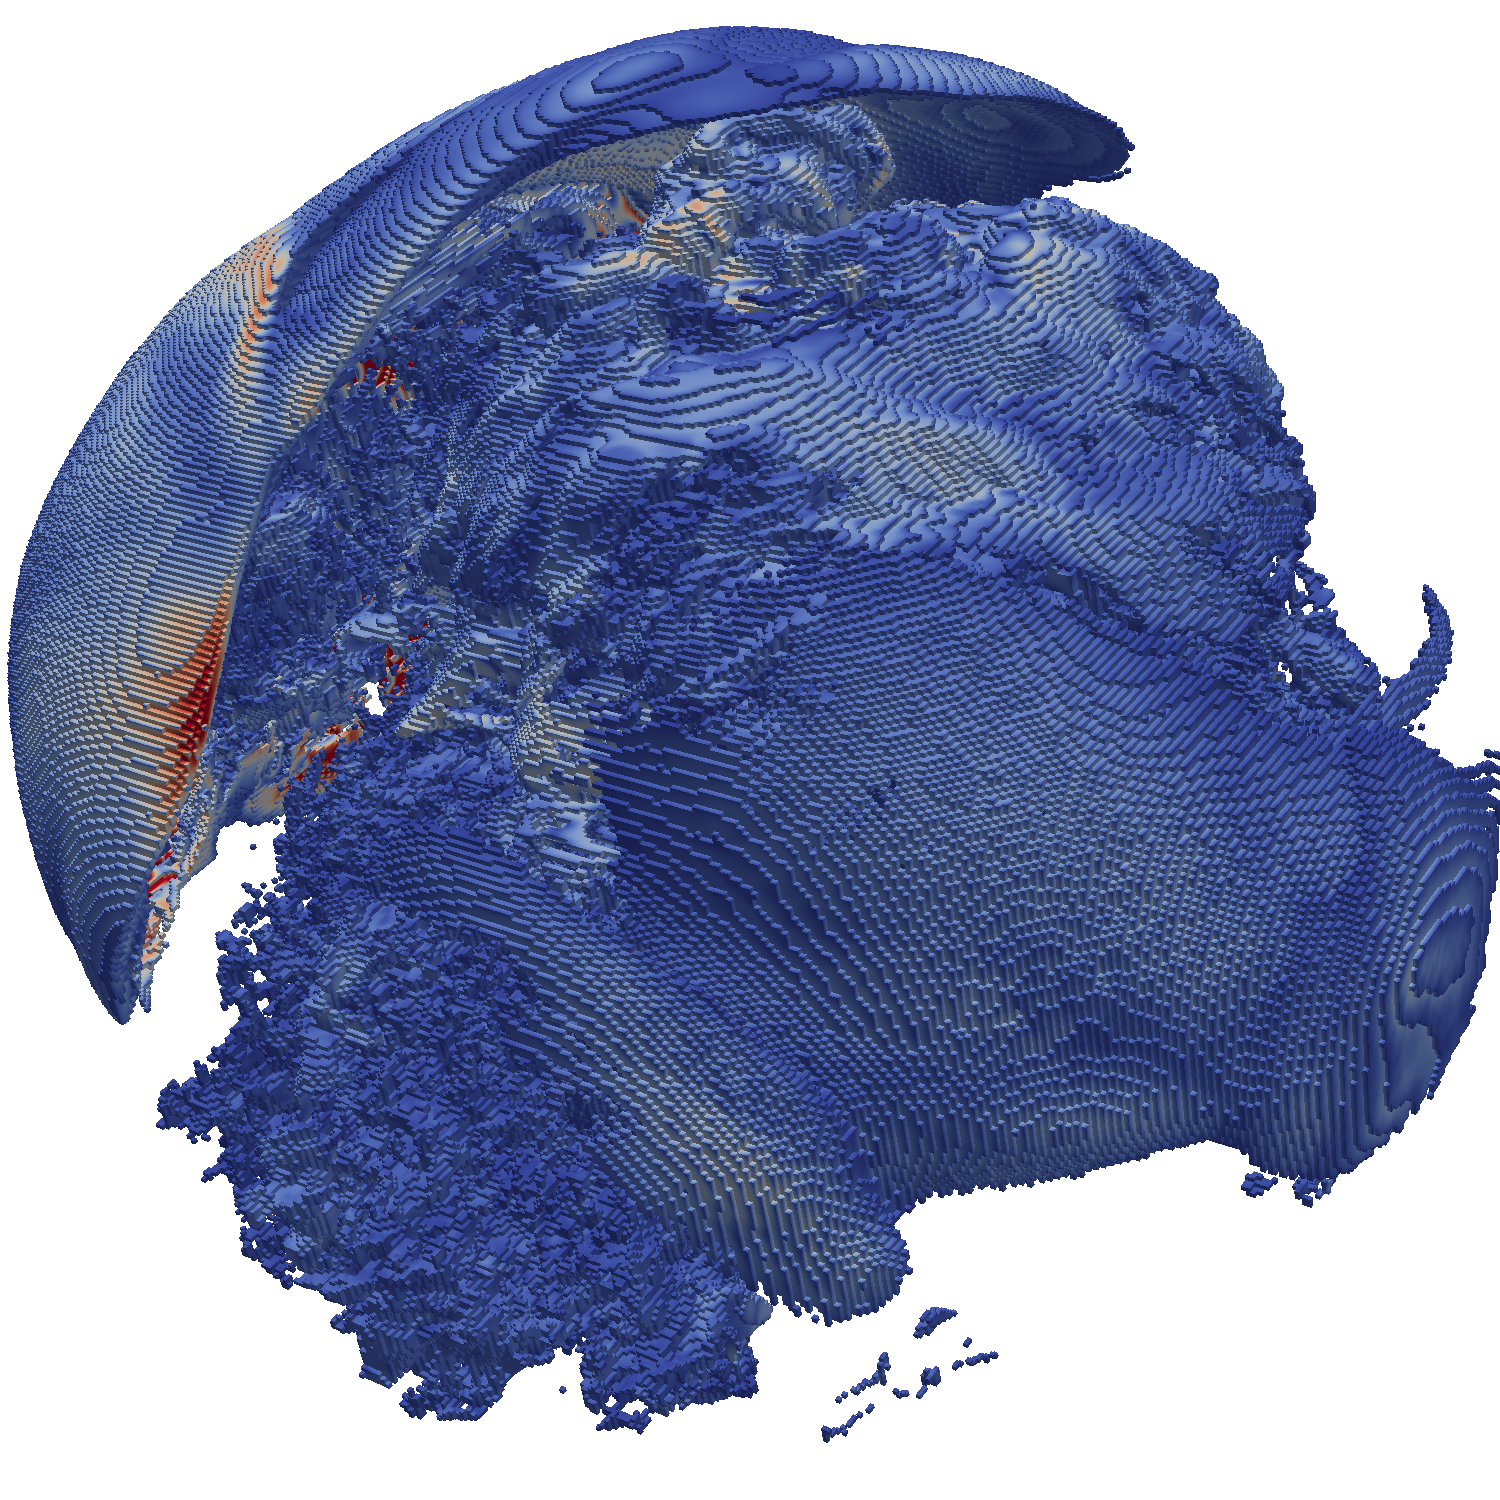
\includegraphics[width=\linewidth]{images/SupernovaThreshold}
  \caption{Supernova dataset used in threshold timing experiments.}
  \label{fig:Supernova}
\end{figure}

\begin{figure*}
  \centering
  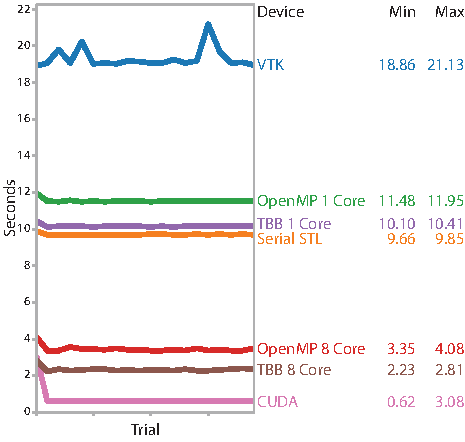
\includegraphics[width=\linewidth]{images/ThresholdTiming}
  \caption{Timing results for threshold operation.}
  \label{fig:Timing}
\end{figure*}

Our threshold algorithm in all instances is run on a large regular mesh
from a supernova simulation made available by John Blondin at the North
Carolina State University and Anthony Mezzacappa of Oak Ridge National
Laboratory\lcite{Blondin2003}.  The data comprises a uniform grid of
$432^3$ points with a 32-bit floating point field value associated with
each point.  The result of our threshold algorithm, shown in
Figure~\ref{fig:Supernova}, contains 3,245,512 cells and 4,090,196 points.
All runs are performed on a Mac desktop with dual Quad-Core Intel Xeon
processors (8 cores total) and 32 GB of system memory.  The system contains
an NVIDIA Quadro 4000 with 2 GB of memory on which CUDA tests were run.

As described in Section~\ref{sec:DeviceAdapter}, Dax's device adapter
mechanism makes it easy to port the toolkit among different execution
environments.  We currently implement three device adapters: a serial
execution that uses the C++ standard template library's algorithms, an
OpenMP execution on multiple CPU cores that uses the Thrust library's
algorithms, and a CUDA execution on NVIDIA GPUs that also uses Thrust.  We
run our Dax threshold algorithm using all three of these device adapters
for comparison purposes.  Because our threshold operation in Dax produces
results that are isomorphic to those produced by VTK, we also run our
algorithm using the VTK filter.  The timing results of all these runs are
summarized in Figure~\ref{fig:Timing}.

First we note that even when Dax is running in serial it outperforms the
VTK implementation.  Because of the large differences between the
implementations of these two algorithms as well as the toolkits they are
in, we cannot draw too many direct conclusions from this comparison.
However, these timings validate the general approach we are talking and
indicate that our generic programming is a viable alternative to the direct
memory access and polymorphic object behavior implemented in VTK.

Because the serial and OpenMP device adapters use different algorithms, we
ran the OpenMP implementation on a single core for comparison purposes.  We
note that the standard template library implementation is significantly
faster than the Thrust implementation.  This might indicate an additional
overhead in the parallel algorithms, or it may indicate that there is room
for improvement in the Thrust implementation.  When the OpenMP
implementation is run using all 8 cores of our system, we see a notable
performance improvement.  We also note that using CUDA to run the threshold
algorithm on the GPU is much faster than any of the multi-core CPU
versions.  This time includes loading data from the CPU into the GPU (but
does not include downloading the results back to the CPU).

\section{Conclusion}
\label{sec:Conclusion}

\noindent
Recent advances in computer architecture represent many opportunities and
challenges for scientific visualization as well as many other fields in
high-performance computing.  Accelerators represent a low-cost, low-power
mechanism to achieve high computation rates.

Because of the diversity of accelerator architectures available, a project
must do better than excel at any one specific system to be successful; it
must adapt itself to a changing landscape of computer architectures.

One of the goals of our Dax project is to provide the flexibility to adjust
to the idiosyncrasies of various processor technologies that might be
available.  We have demonstrated that it is possible through generic
programming to adapt to a variety of programming environments with little
overhead.

\section*{Acknowledgments}

\noindent
This work was supported in whole by the DOE Office of Science, Advanced
Scientific Computing Research, under award number 10-014707, program
manager Lucy Nowell.

Sandia National Laboratories is a multi-program laboratory operated by
Sandia Corporation, a wholly owned subsidiary of Lockheed Martin
Corporation, for the U.S. Department of Energy's National Nuclear Security
Administration.

\bibliographystyle{IEEEtranS}
\bibliography{DaxPDAC2012}

\end{document}
